\section{Lecture 3: Linear Algebra I}

Most, if not all, algebra learned throughout K-12 educations deals with \emph{scalar} algebra. Each variable only represents a single number. But, a variable can represent more than one element. Instead:

\begin{itemize}
    \item \emph{Scalar}: one element, $x$
    \item \emph{Vector}: $n$ elements
    \begin{itemize}
        \item $\bm{x}$ includes the set of scalars $x_1, x_2, ..., x_i,..., x_n$
    \end{itemize}
    \item \emph{Matrix}: $n \times m$ elements
    \begin{itemize}
        \item $\bm{X}$ include the set of scalars 
        $x_{11},..., x_{1m}, x_{21},..., x_{2m}, ..., x_{n1},..., x_{nm}$
    \end{itemize}
\end{itemize}

\noindent There are considerable gains to be made through this notation. Beyond a more efficient notation, we're able to easily carry out all sorts of useful manipulations. We'll work up to these benefits in this lecture through various concepts.

\subsection{Systems of equations}

\begin{itemize}
    \item \emph{System of equations}: two or more equations with the same variables
    \begin{itemize}
        \item To find a unique solution, we need as many equations as variables. E.g.,
        \begin{align*}
            6x_1 & - 3x_2 + 4x_3 = -13 \\
            6x_1 & = -13 + 3x_2 - 4x_3 \\
            x_1  & = -\frac{13}{6} + \frac{1}{2}x_2 - \frac{2}{3}x_3
        \end{align*} 
        \item We can use this single equation and solution to create a series of solutions, i.e. if $x_2 = 2$ and $x_3 = 3$, then $x_1 = -\frac{13}{6}$ and so on.
    \end{itemize}
\end{itemize}

\begin{itemize}
    \item Consider the following system of (linear) equations:
    \begin{align*}
        a_{11}x_1 + a_{12}x_2 + a_{13}x_3 + ... + a_{1n}x_n & = b_1 \\
        a_{21}x_1 + a_{22}x_2 + a_{23}x_3 + ... + a_{2n}x_n & = b_2 \\
        & \vdots \\
        a_{m1}x_1 + a_{m2}x_2 + a_{m3}x_3 + ... + a_{mn}x_n & = b_m 
    \end{align*}
    Drawing on yesterday's lecture, we can also write this all as: $\sum\limits_{i = 1}^m\sum\limits_{j = 1}^n a_{ij}x_j = b_i$ Or, bringing matrix notation in, as: $\bm{A}\bm{x} = \bm{b}$, where $\bm{A}$ is an $n \times m$ matrix.
\end{itemize}

\subsubsection{Solving for a system of equation}

Consider the following system of equations. Throughout $r$ references row number. By setting all variables but one per equation, we are solving by \emph{elimination}. We'll later introduce Gauss-Jordan elimination, which is the same process, but with an augmented matrix.

\begin{itemize}
    \item First, the equations:
    \begin{align*}
        1x_1 + 1x_2 & = 100,000 \\
        0.05x_1 + 0.09x_2 & = 7,800        
    \end{align*}
    \item Add $-0.05r1$ to $r2$
    \begin{align*}
        1x_1 + 1x_2 & = 100,000 \\
        0x_1 + 0.04x_2 & = 2,800        
    \end{align*}
    \item $25r2$
    \begin{align*}
        1x_1 + 1x_2 & = 100,000 \\
        0x_1 + 1x_2 & = 70,000        
    \end{align*}
    \item Subtract r2 from r1 
    \begin{align*}
        1x_1 + 0x_2 & = 30,000 \\
        0x_1 + 1x_2 & = 70,000
    \end{align*}
    \item This gives us: $x_1 = 30,000$ and $x_2 = 70,000$
\end{itemize}

\noindent Now, let's try a lengthier example. Again, we're not substituting equations into each variable. We're eliminating all variables but one from each equation.

\begin{itemize}
    \item First, the equations:
    \begin{align*}
        1x_1 + 2x_2 + 3x_3 & = 6 \\
        2x_1 - 3x_2 + 2x_3 & = 14 \\
        3x_3 + 1x_2 - 1x_3 & = -2 
    \end{align*}
    \item Subtract $-2r1$ from $r2$ and subtract $-3r1$ from $r3$
    \begin{align*}
        1x_1 + 2x_2 + 3x_3 & = 6 \\
        0x_1 - 7x_2 - 4x_3 & = 2 \\
        0x_3 - 5x_2 - 10x_3 & = -20
    \end{align*}
    \item Multiply $r3$ by $-\frac{1}{5}$ and flip $r2$ and $r3$
    \begin{align*}
        1x_1 + 2x_2 + 3x_3 & = 6 \\
        0x_1 + 1x_2 + 2x_3 & = 4 \\
        0x_3 - 7x_2 - 4x_3 & = 2
    \end{align*}
    \item Subtract $2r2$ from $r1$ and add $7r2$ to $r3$
    \begin{align*}
        1x_1 + 0x_2 - 1x_3 & = -2 \\
        0x_1 + 1x_2 + 2x_3 & = 4 \\
        0x_3 + 0x_2 + 10x_3 & = 30
    \end{align*}
    \item Divide $r3$ by 10
    \begin{align*}
        1x_1 + 0x_2 - 1x_3 & = -2 \\
        0x_1 + 1x_2 + 2x_3 & = 4 \\
        0x_3 + 0x_2 + 1x_3 & = 3
    \end{align*}
    \item Add $r3$ to $r1$ and subtract $2r3$ from $r2$
    \begin{align*}
        1x_1 + 0x_2 - 0x_3 & = 1 \\
        0x_1 + 1x_2 + 0x_3 & = -2 \\
        0x_3 + 0x_2 + 1x_3 & = 3
    \end{align*}
    \item $x_1 = 1, x_2 = -2, x_3 = 3$
\end{itemize}

\noindent Writing all of the $x's$ gets tedious though. So let's introduce vectors.

\subsection{Vectors}

\begin{itemize}
    \item Examples:
    \begin{itemize}
        \item $\bm{x} = [x_1, x_2, x_3, ..., x_n]$
        \item $\bm{x} = (5, 2)$
        \begin{itemize}
            \item If, like in this case, there are two dimensions (number of components), then we can visually understand the vector as:
            
            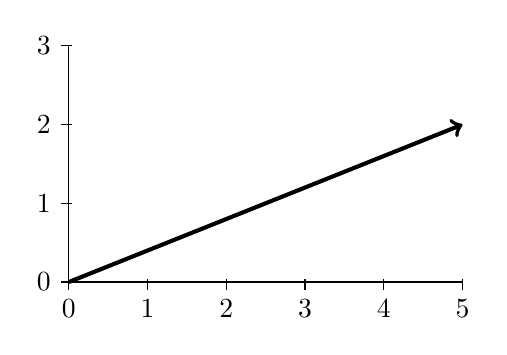
\begin{tikzpicture}
                %axis
                \draw (0,0) -- coordinate (x axis mid) (5,0);
                    \draw (0,0) -- coordinate (y axis mid) (0,3);
                    %ticks
                    \foreach \x in {0,...,5}
                        \draw (\x,1pt) -- (\x,-3pt)
                        node[anchor=north] {\x};
                    \foreach \y in {0,...,3}
                        \draw (1pt,\y) -- (-3pt,\y) 
                        node[anchor=east] {\y};
                \draw   (5,0) -- (0, 0)
                        (0,3) -- (0,0);
                \draw[->,line width=1.5pt] (0,0) -- (5,2);
            \end{tikzpicture}
        
        \end{itemize}

    \item If we multiply by a scalar: $a = 2$, $aX = [10, 4]$
    
    \begin{tikzpicture}
        %axis
        \draw (0,0) -- coordinate (x axis mid) (10,0);
            \draw (0,0) -- coordinate (y axis mid) (0,5);
            %ticks
            \foreach \x in {0,...,10}
                \draw (\x,1pt) -- (\x,-3pt)
                node[anchor=north] {\x};
            \foreach \y in {0,...,5}
                \draw (1pt,\y) -- (-3pt,\y) 
                node[anchor=east] {\y};
        \draw   (10,0) -- (0, 0)
                (0,5) -- (0,0);
        \draw[->,line width=1.5pt] (0,0) -- (5,2);
        \draw[->,line width=1.5pt] (0,0) -- (10,4);
    \end{tikzpicture}

    \end{itemize}
\end{itemize}

\subsubsection{Vector length}

\begin{itemize}
    \item Also called the \emph{norm}, length is not the same as \emph{dimensions}. The formula is:

    \begin{equation*}
        ||x|| = \sqrt{x_1^2 + x_2^2 + ... + x_n^2}
    \end{equation*}

    \item Considering the visuals above, in two dimensions we are just using the Pythagorean theorem. But the formula is extendable to k-dimensions. For $\bm{x} = (5, 2)$, $||\bm{x}|| = \sqrt{25 + 4} = \sqrt{29}$.
    
    \item Another example
    \begin{itemize}
        \item $x = (5,2), y = (1,4)$
        \begin{itemize}
            \item $x + y = (6, 6)$
            \item $||x + y|| = \sqrt{36 + 36} = \sqrt{72}$
        
            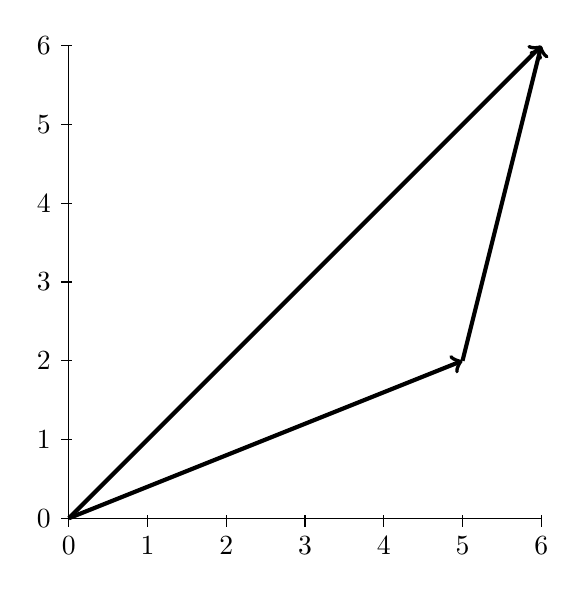
\begin{tikzpicture}
                %axis
                \draw (0,0) -- coordinate (x axis mid) (6,0);
                    \draw (0,0) -- coordinate (y axis mid) (0,6);
                    %ticks
                    \foreach \x in {0,...,6}
                        \draw (\x,1pt) -- (\x,-3pt)
                        node[anchor=north] {\x};
                    \foreach \y in {0,...,6}
                        \draw (1pt,\y) -- (-3pt,\y) 
                        node[anchor=east] {\y};
                \draw   (6,0) -- (0, 0)
                        (0,6) -- (0,0);
                \draw[->,line width=1.5pt] (0,0) -- (5,2);
                \draw[->,line width=1.5pt] (5,2) -- (6,6);
                \draw[->,line width=1.5pt] (0,0) -- (6,6);
            \end{tikzpicture}
        \end{itemize}
    \end{itemize}

    %\item One side note on distance:
    %\begin{itemize}
    %    \item The \emph{triangle inequality} states that:
    %    \begin{itemize}
    %        \item $||x + y|| \leq ||x|| + ||y||$
    %    \end{itemize}
    %\end{itemize}
\end{itemize}

\subsubsection{Vector multiplication}

\begin{itemize}
    \item If $c$ is a \emph{scalar} and we multiply $a(x_1, x_2, ..., x_n)$, then we get $(ax_1, ax_2, ..., ax_n)$. Dividing by a scalar works the same way.
    \item But what about multiplying one vector by another vector? We use the \textbf{dot product}: $\bm{a} \cdot \bm{b}$. Another name for this operation is the \textbf{inner product}.\footnote{For a nice review of vector manipulation, see \url{https://people.cs.clemson.edu/~dhouse/courses/401/notes/vectors.pdf}}
    \begin{itemize}
        \item If $\bm{a}$ and $\bm{b}$ are both n-dimensional, then $\bm{a} \cdot \bm{b} = a_1b_1 + a_2b_2 + ... + a_nb_n = \sum\limits_{i=1}^na_ib_i$
        \begin{equation*}
            \text{Ex: }
            \begin{bmatrix}
                5 \\
                2
            \end{bmatrix} \cdot 
            [1 \; \; 4]
            = (5 \cdot 1) + (2 \cdot 4) = 5 + 8 = 13  
        \end{equation*}
        \item Note: the result of the dot product of vectors is a \emph{scalar}.
    \end{itemize}
    %\item The \textbf{Cauchy-Schwartz inequality} states that $|a \cdot b| %\leq ||a|| \, ||b||$
    \item The \textbf{outer product} of two vectors instead produces a matrix:
    \begin{equation*}
        \begin{bmatrix}
            a_1 \\
            a_2
        \end{bmatrix} \cdot 
        \begin{bmatrix}
            b_1 & b_2
        \end{bmatrix}
        = \begin{bmatrix}
            a_1b_1 & a_1b_2 \\
            a_2b_1 & a_2b_2
        \end{bmatrix}  
    \end{equation*}
    \begin{itemize}
        \item The dimensions of this matrix are the two outer dimensions of the vectors multiplied together:
        \begin{equation*}
            \underset{3 \times 1}{\begin{bmatrix}
                3 \\
                2 \\
                1
            \end{bmatrix}}
            \underset{1 \times 3}{[1 \; \; 2 \; \; 3]} = 
            \underset{3 \times 3}{
            \begin{bmatrix}
                3 & 6 & 9 \\
                2 & 4 & 6 \\
                1 & 2 & 3
            \end{bmatrix}
            }
        \end{equation*}
        \item \emph{But} the inner dimensions must match up. See 1 and 1 above. If the first matrix's number of columns is not equal to the second matrix's number of rows, then cannot multiply.
    \end{itemize}
\end{itemize}

% Take lecture break here
\subsection{Matrices}

\begin{itemize}
    \item A \textbf{matrix} is a rectangular table of numbers or variables arranged in a specific order in rows and columns. We express dimensions by rows, $n$, and columns, $m$. The dimensions of a matrix $A_{n \times m}$ are pronounced `$n$ by $m$'. 
    
    \begin{equation*}
        \bm{X} = 
        \begin{bmatrix}
            x_{11} & x_{12} & x_{13} \\
            x_{21} & x_{22} & x_{23} \\
            x_{31} & x_{32} & x_{33} 
        \end{bmatrix} \in
        \mathbb{R}^{nm} = \mathbb{R}^{3 \times 3}
    \end{equation*}

    \item If $m = n$, then the matrix is symmetric/square.
    
    \item \textbf{Types of matrices}:
    \begin{equation*}
        \begin{bmatrix}
            0 & 0 & 0 \\
            0 & 0 & 0 \\
            0 & 0 & 0
        \end{bmatrix} = \text{zero matrix}
        \; \; \; \;
        \begin{bmatrix}
            1 & 0 & 0 \\
            0 & 2 & 0 \\
            0 & 0 & 3
        \end{bmatrix} = \text{diagonal matrix}
        \; \; \; \; 
        \begin{bmatrix}
            1 & 0 & 0 \\
            0 & 1 & 0 \\
            0 & 0 & 1
        \end{bmatrix} = \text{identity matrix}
    \end{equation*}
\end{itemize}

\subsection{Matrix operators}

\begin{itemize}
    
    \item \textbf{Addition}
    
    \begin{itemize}
        \item Must have the same number of elements
        \begin{equation*}
            \begin{bmatrix}
                1 & 2 & 3 \\
                0 & 0 & 1 \\
                1 & 2 & 1
            \end{bmatrix} +
            \begin{bmatrix}
                1 & 2 \\
                3 & 4 \\
                5 & 6
            \end{bmatrix} = \text{can't do}
        \end{equation*}
        \begin{equation*}
            \begin{bmatrix}
                1 & 2 \\
                0 & 0 \\
                1 & 2
            \end{bmatrix} + 
            \begin{bmatrix}
                1 & 2 \\
                3 & 4 \\
                5 & 6
            \end{bmatrix} =
            \begin{bmatrix}
                2 & 4 \\
                3 & 4 \\
                6 & 8
            \end{bmatrix}
        \end{equation*}
    \end{itemize}

    \item \textbf{Transposition}
    
    \begin{itemize}
        \item Rotate so that the first column becomes the first row:
        \begin{equation*}
            \bm{X} = 
            \underset{3 \times 2}{
            \begin{bmatrix}
                1 & 2 \\
                0 & 0 \\
                1 & 2    
            \end{bmatrix}
            }, 
            \; \; \; 
            \bm{X}^T = 
            \underset{2 \times 3}{
            \begin{bmatrix}
                1 & 0 & 1 \\
                2 & 0 & 2   
            \end{bmatrix}
            }
        \end{equation*}
    \end{itemize} 

    \item \textbf{Multiplication}
        \begin{align*}
            \bm{A} = 
            \begin{bmatrix}
                1 & 2 \\
                3 & 4    
            \end{bmatrix},
            \; \; \; 
            \bm{B} =
            \begin{bmatrix}
                7 & 0 & -1 \\
                1 & 3 & 1
            \end{bmatrix}
        \end{align*}
        
        \begin{itemize}
            \item Because $\bm{A}$ is $2 \times 2$ and $\bm{B}$ is $2 \times 3$, we can multiply. But $\bm{A}\bm{B}^T$ is undefined because $\bm{B}$ is $3 \times 2$. 
        \end{itemize}
        \begin{align*}
            \bm{AB} & =
            \begin{bmatrix}
                1 & 2 \\
                3 & 4
            \end{bmatrix}
            \begin{bmatrix}
                7 & 0 & -1\\
                1 & 3 & 1
            \end{bmatrix} \\
            & = 
            \begin{bmatrix}
                \bm{A}_{11}\bm{B}_{11} + \bm{A}_{12}\bm{B}_{21} & 
                \bm{A}_{11}\bm{B}_{12} + \bm{A}_{12}\bm{B}_{22} &
                \bm{A}_{11}\bm{B}_{13} + \bm{A}_{12}\bm{B}_{23} \\ 
                \bm{A}_{21}\bm{B}_{11} + \bm{A}_{222}\bm{B}_{21} & 
                \bm{A}_{21}\bm{B}_{12} + \bm{A}_{22}\bm{B}_{22} &
                \bm{A}_{21}\bm{B}_{13} + \bm{A}_{22}\bm{B}_{23}
            \end{bmatrix} \\
            & =
            \begin{bmatrix}
                (1 \cdot 7) + (2 \cdot 1) & 
                (1 \cdot 0) + (2 \cdot 3) &
                (1 \cdot -1) + (2 \cdot 1) \\ 
                (3 \cdot 7) + (4 \cdot 1) &
                (3 \cdot 0) + (4 \cdot 3) & 
                (3 \cdot -1) + (4 \cdot 1) 
            \end{bmatrix} 
            = 
            \begin{bmatrix}
                9 & 6 & 1 \\
                29 & 12 & 1
            \end{bmatrix}
        \end{align*}

    \begin{itemize}
        \item Ex with identity matrix:
        \begin{align*}
            \bm{I}_{2 \times 2} \bm{X} & = 
            \begin{bmatrix}
                1 & 0 \\
                0 & 1
            \end{bmatrix}
            \begin{bmatrix}
                1 & 2 \\
                3 & 4
            \end{bmatrix} = 
            \begin{bmatrix}
                1 & 2 \\
                3 & 4
            \end{bmatrix} \\
            & 
            \text{b/c}
            \begin{bmatrix}
                (1 \cdot 1) + (0 \cdot 3) & (0 \cdot 1) + (1 \cdot 2) \\
                (0 \cdot 1) + (1 \cdot 3) & (0 \cdot 3) + (1 \cdot 4) 
            \end{bmatrix}
        \end{align*}
    \end{itemize}

\end{itemize}